\subsection*{Il software Mantis}
Per segnalare gli errori o le richieste di intervento in modo che vengano visualizzati e gestiti dagli sviluppatori 
� necessario accedere alla pagina: 

\url{http://mantis.comune.intranet/}

Dalla quale si viene come al solito rimandati alla pagina di autenticazione.

\begin{flushleft}
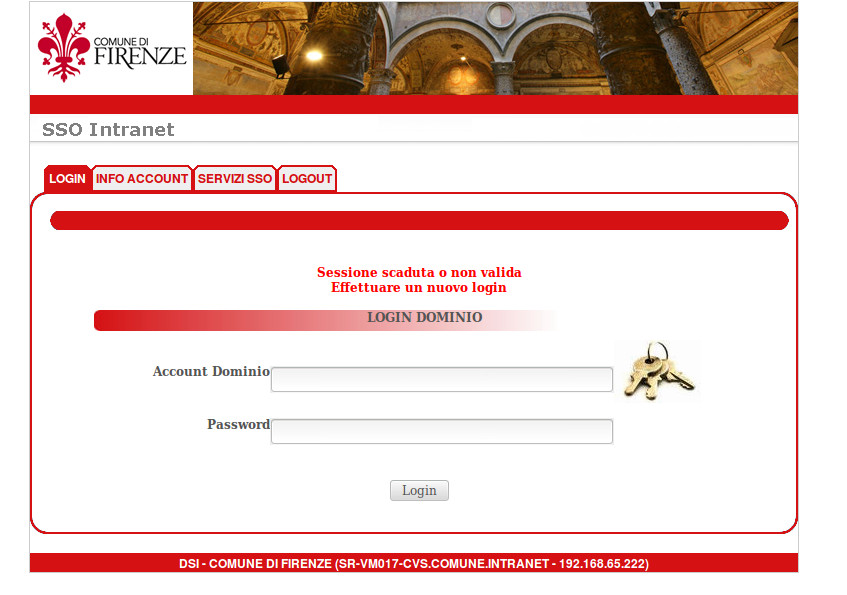
\includegraphics[scale=0.7]{img_mantis/001_sso.jpg}
\end{flushleft}

Se si era gi� autenticati o se il ci si � autenticati il programma rimanda alla pagina iniziale di Mantis. 

\begin{flushleft}
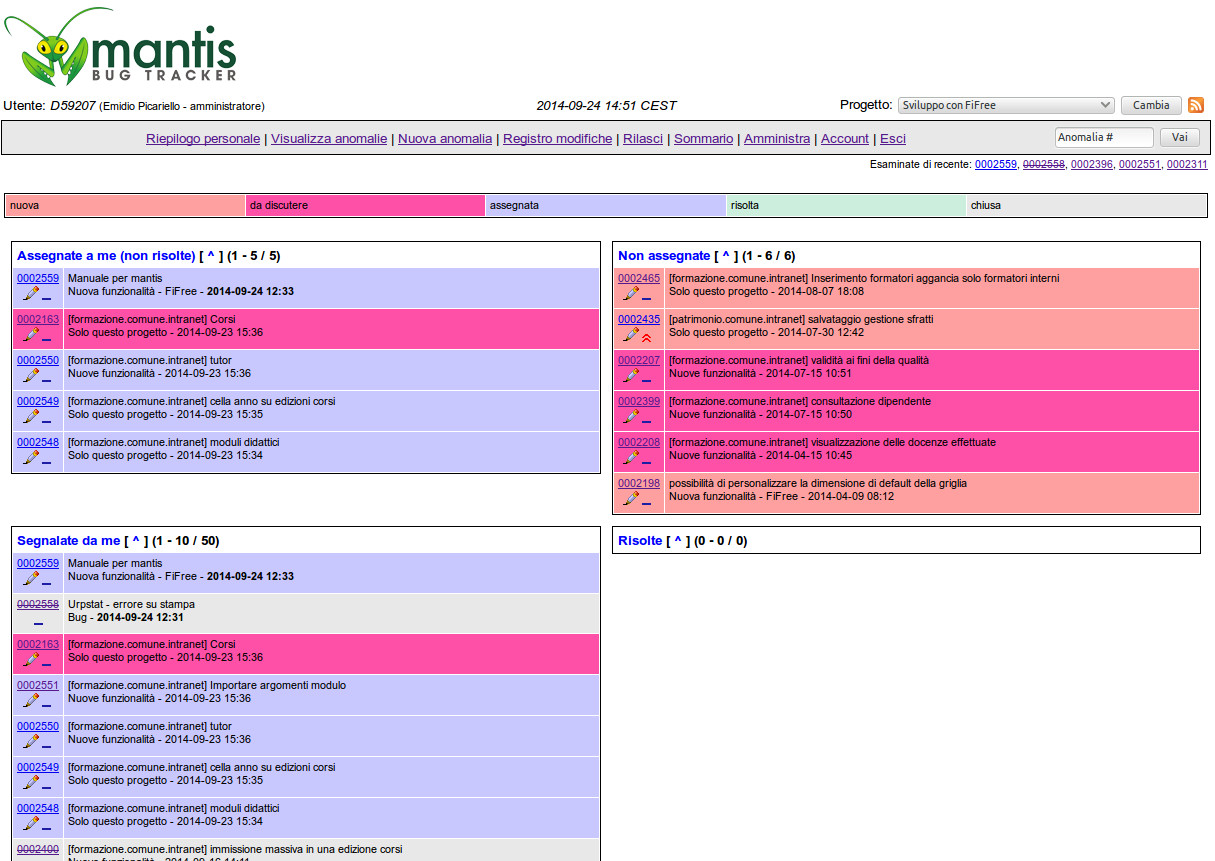
\includegraphics[scale=0.5]{img_mantis/010_home.jpg}
\end{flushleft}

Se non si � indirizzati a questa pagina, scrivere una mail a \var{mail_assistenza} indicando il proprio numero di matricola, il proprio nome
la propria email completa e il programma per il quale si vuole essere abilitati alla segnalazione di errori o migliorie. \\

La pagina che ci si trova di fronte ha in alto a destra il nome del progetto (se siete abilitati a pi� progetti scegliete l� per quale progetto 
state facendo la segnalazione). 

\begin{flushleft}
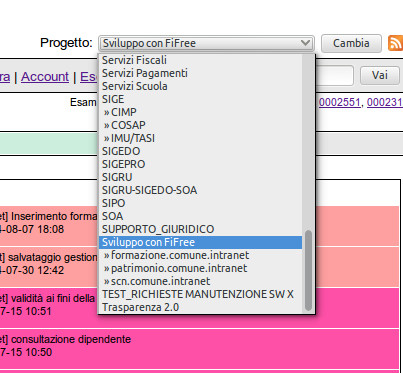
\includegraphics[scale=0.7]{img_mantis/020_progetto.jpg}
\end{flushleft}

Nel corpo della pagina vedrete le segnalazioni che avete fatto e il loro stato, indicato dal colore: 

\begin{flushleft}
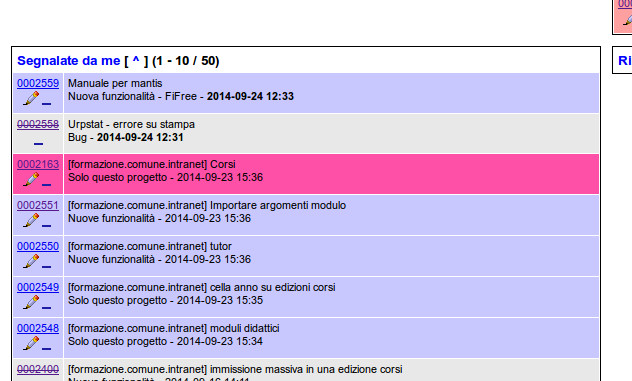
\includegraphics[scale=0.7]{img_mantis/030_segnalate.jpg}
\end{flushleft}

Nel men� avete invece la possibilit� di cliccare su \virgolette{Nuova Anomalia} che apre la pagina nella quale potete immettere la nuova 
richiesta: 

\begin{flushleft}
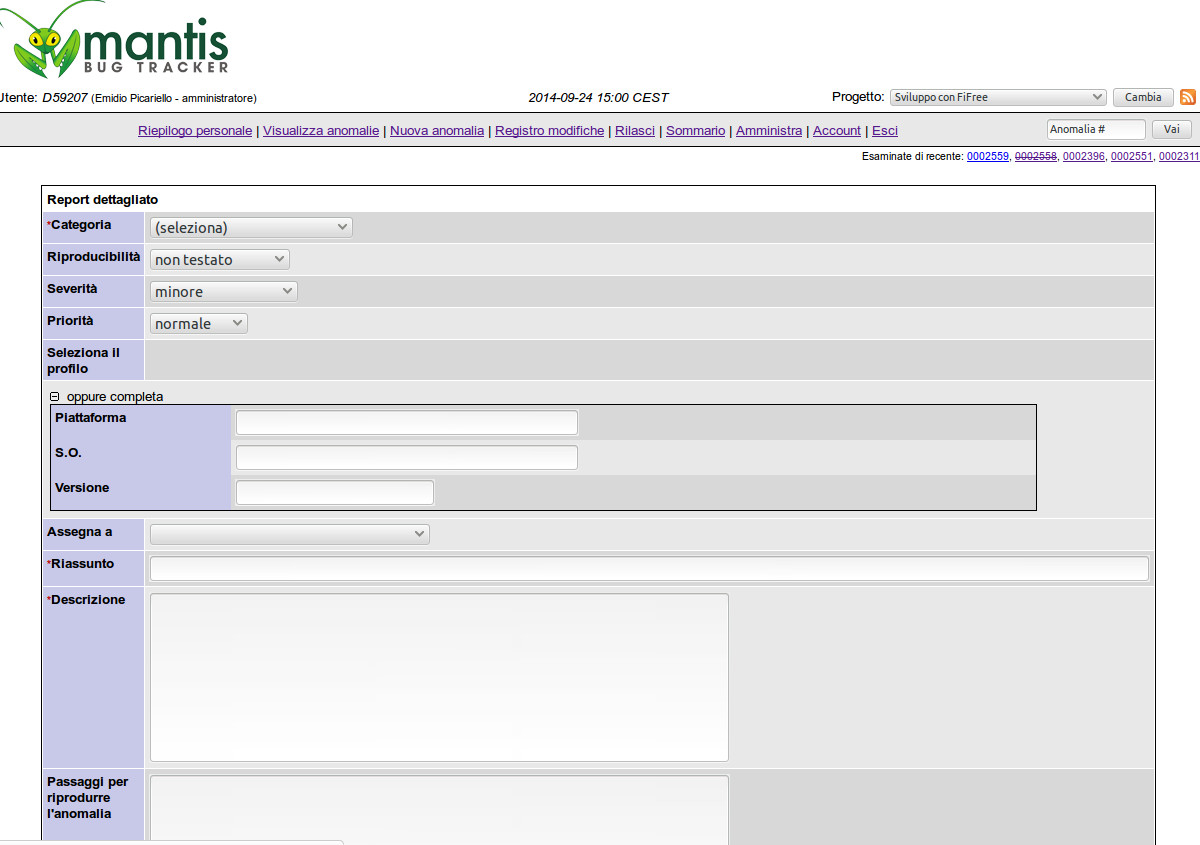
\includegraphics[scale=0.5]{img_mantis/050_segnala.jpg}
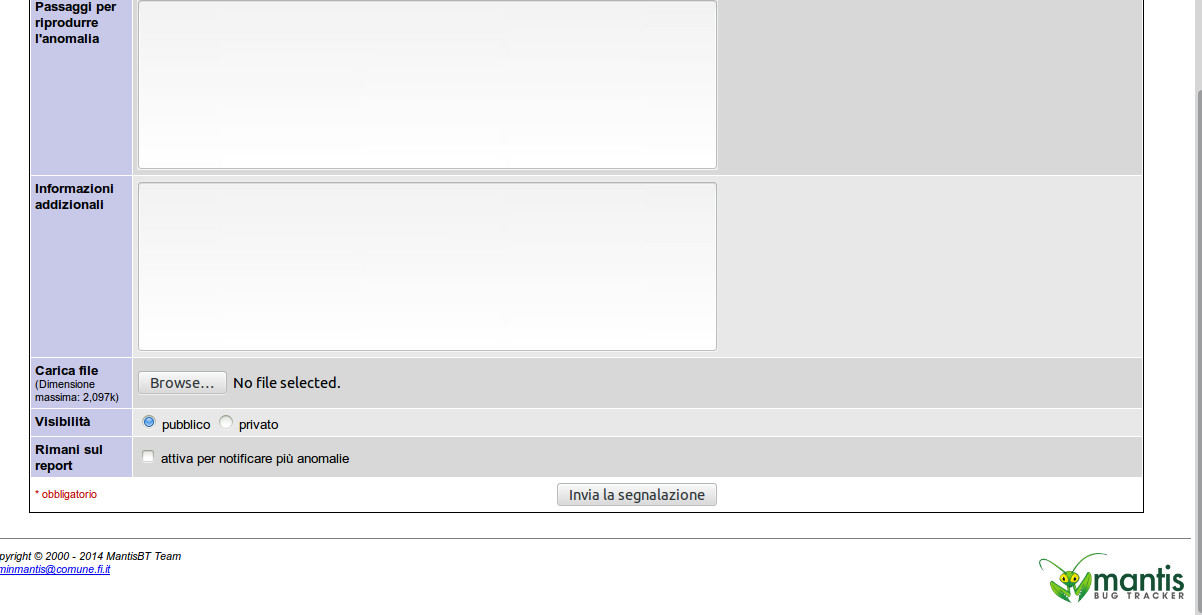
\includegraphics[scale=0.5]{img_mantis/055_segnala.jpg}
\end{flushleft}

I campi contrassegnati dall'asterisco sono obbligatori. Per fare una buona segnalazione � necessario ragionare attentamente sulle 
informazioni che si forniscono e su quelle che si omettono. Nel campo \virgolette{categoria}si sceglie la categoria pi� appropriata 
fra quelle che sono disponibili per il progetto. Nel campo \virgolette{riproducibilit�} si 
segnala se l'errore si verifica tutte le volte che si fa una determinata operazione o se si verifica solo ogni tanto 
o se si � verificato una volta ma non si � in grado di riprodurlo. I due campi successivi sono diversi e molto importanti: 
la \virgolette{severit�} di un errore ha a che fare con quanto grave �. Le voci sono in ordine di gravit�, \virgolette{crash} significa
che il programma si chiude quando si verifica quell'errore, \virgolette{blocco} significa che non c'� modo di andare avanti. 
Il campo \virgolette{priorit�} invece indica quanto urgente � l'errore o la richiesta. Chiaramente ci deve essere un grado. 
Se tutte le richieste sono segnalate come \virgolette{immediata} o \virgolette{urgente} chi deve farsene carico non sapr� da quale cominciare. 
Per esempio: se lancio una stampa una volta l'anno e i dati di quella stampa sono sbagliati, l'errore sar� di gravit� \virgolette{maggiore} 
ma la priorit� sar� \virgolette{normale}. \\
I dati relativi a piattaforma e sistema operativo si possono normalmente omettere a meno che non si debba comunicare qualcosa che il programmatore non 
sa (i programmi si usano con Firefox su Windows, se ho un Mac e uso Safari, lo devo scrivere qui). \\
Il riassunto deve essere breve e indicare che cosa accade, invece nella descrizione � importante scrivere dove ci si trova (per esempio) 
\virgolette{Tabelle} $\rightarrow$ \virgolette{Anagrafiche}. Se si scrive per esempio \virgolette{non controlla la data} questo sar� un errore impossibile da correggere. 
Che vuol dire? Cosa dovrebbe controllare? In che pagina si verifica l'errore? Invece \virgolette{in anagrafica cliente non controlla che la 
data di nascita sia anteriore a 18 anni fa per verificare che il soggetto immesso abbia la maggiore et�} � un errore segnalato correttamente. 
Pi� i dati sono corretti e completi e pi� veloce sar� la risoluzione del problema. \\
Una volta immessi tutti i dati basta cliccare su \virgolette{Invia la segnalazione} 